\documentclass{article}
\usepackage[utf8]{inputenc}

\title{Relazione Progetto Algoritmi}
\author{Koci Erik}
\date{September 2021}

\usepackage{natbib}
\usepackage{graphicx}
\usepackage{listings}   
\usepackage{tcolorbox}
% Include the listings-package
\lstset{breaklines}

\begin{document}

\maketitle
\section{Intestazione}
\textbf{Nome del progetto:} Progetto ASD A.A. 2020-2021 (M,N,K)-game\\
\textbf{cognome e nome autore:} Koci Erik\\
\textbf{Matricola:} 0000997662

\section{Problema}
\begin{itemize}
    \item Sviluppare un giocatore software in grado di giocare in modo ottimale a tutte le istanze possibili del (M,N,K)-game.
    \item Il numero di mosse intelligenti cresce esponenzialmente rispetto alla dimensione della matrice di gioco ed il numero di simboli da allineare.
    \item Tramite una dimostrazione per furto di strategia si può dimostrare che il secondo giocatore non può avere una strategia che gli assicuri la vittoria.
\end{itemize}

\begin{figure}[h!]
\centering
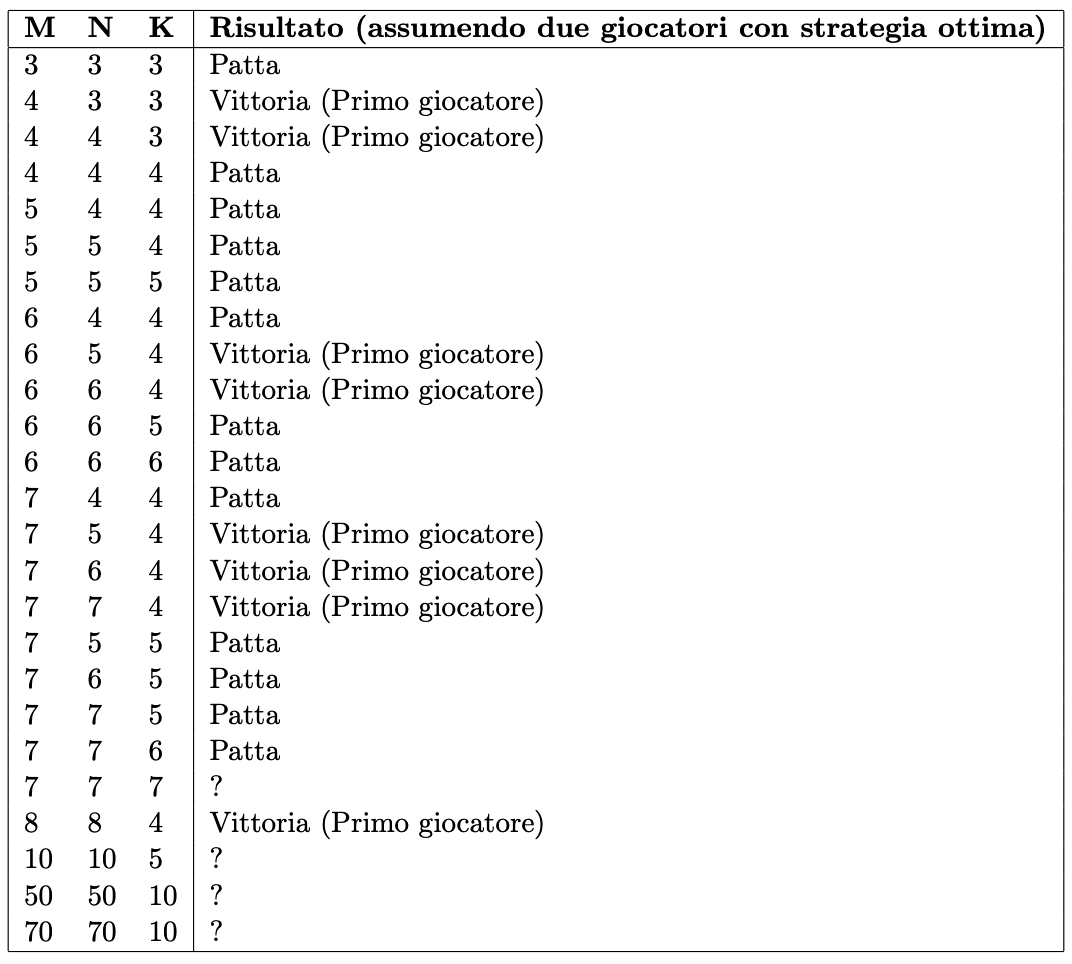
\includegraphics[width=8cm,height=6cm]{match.png}
\caption{Esempi di configurazione m,n,k}
\label{fig:universe}
\end{figure}

\section{Scelte progettuali}
    Nello sviluppo progettuale del metodo \textbf{selectCell()} inizialmente ho utilizzato l'algoritmo noto di ricerca \textbf{alpha-beta pruning}, il quale riduce notevolmente il numero di mosse da valutare nel gioco in questione. Questa tipologia di algoritmo viene spesso utilizzata nei giochi a turni tra due o più giocatori.
    \subsection{Funzionamento dell'algoritmo}
    L'algoritmo \textbf{alpha-beta pruning} si basa principalmente su due valori, \textbf{alpha} e \textbf{beta}, i quali in ogni punto dell'albero, rappresentano la posizione migliore e peggiore che è possibile raggiungere. Se \textbf{A} è il giocatore \textbf{massimizzante} e \textbf{B} il giocatore \textbf{minimizzante} accade che:
    \begin{itemize}
        \item $\alpha$ è il punteggio minimo che \textbf{A} può raggiungere, a partire dalla posizione in esame; all'inizio dell'algoritmo viene posto a -$\infty$. Durante il calcolo, $\alpha$ coincide con il valore della \textbf{migliore mossa} possibile attualmente calcolata per \textbf{A}.
        \item $\beta$ è il punteggio massimo che \textbf{B} può raggiungere a partire dalla stessa posizione; all'inizio dell'algoritmo viene posto a +$\infty$. Durante il calcolo, $\beta$ coincide con il valore della \textbf{migliore mossa} possibile attualmente calcolata per \textbf{B}.
    \end{itemize}
    
    Se durante la ricerca, per un dato nodo $\alpha$ diventa \textbf{maggiore} di $\beta$, la \textbf{ricerca} al di sotto di quel nodo \textbf{cessa} e il programma passa ad un altro sottoalbero perché da quella posizione in poi, A \textbf{perderebbe} anche se giocasse per vincere. \citep{alpha-beta-pruning}
    Una volta terminata una eseguzione di gioco, la funzione \texttt{evaluate} determinerà il punteggio da attribuire a seconda del \texttt{game state}.
   
    \\
    \begin{figure}[h!]
    \centering
    \includegraphics[width=10cm,height=6cm]{alphaBetaPruning.png}
    \caption{alpha-beta Pruning}
    \label{fig:universe}
    \end{figure}
    
    \newpage
    \subsection{Complessità computazionale}
    
    Con un fattore di ramificazione \textbf{b} e una profondità di ricerca di \textbf{d} strati, quando l'ordine di spostamento è \textbf{pessimo} la complessità computazionale  è $O(b\cdot b\cdot ...\cdot b) = O(b^d)$.\\
    Se l'ordine delle mosse per la ricerca è \textbf{ottimale}, il numero di posizioni del nodo foglia valutate è circa $O(b \cdot 1 \cdot b \cdot 1 \cdot ... \cdot b)$ per profondità dispari è $O(b \cdot 1 \cdot b \cdot 1 \cdot ... \cdot 1)$ per una profondità uniforme  $O(b^d^/^2) = O(\sqrt{b^d})$.\\
    In quest'ultimo caso, dove la tela di una ricerca è pari, il fattore di ramificazione effettivo è ridotto alla sua \textbf{radice quadrata}.
 \citep{alpha-beta}
    \\\\
    \textbf{Worst-case performance:} $O(b^d)$
    \\
    \textbf{Best-case performance:} $O(\sqrt{b^d})$

    \subsubsection{Pseudocodice:}
    \lstset{language=java, numbers=left,numbersep=8pt,  }
    \begin{lstlisting}[frame=single]  
function alphabeta(node,depth,a,b,maximizingPlayer) {
 if depth = 0 or node is a terminal node then
   return the heuristic value evaluate(value)
   if maximizingPlayer then
     value := -infinity
     for each goodMoves do
       value := max(value,alphabeta(child,depth-1,a,b,false))
       a := max(a,value)
       if value >= b then
         break (* b cutoff *)
         return value
    else
      value := +infinity
      for each goodMoves do
        value := min(value,alphabeta(child,depth-1,a,b,true))
        b := min(b,value)
        if value <= a then
          break (* a cutoff *)
      return value
}
    \end{lstlisting}
    
        \lstset{language=java}
    \begin{lstlisting}[frame=single]  
function evaluate(MNKBoard B) {
    if(state == OPEN) return 1;
    else if(state == DRAW) return 0;
    else if(state == myWin) return 10;
    else return -10;
}
    \end{lstlisting}
    
    \subsection{strategie nell’implementazione}
    A livello di strategie di implementazione, oltre all'\textbf{euristica} dell'algoritmo citato precedentemento, ho utilizzato anche altre tre funzioni, le quali ci permettono di:
    \begin{enumerate}
        \item Ricavare e analizzare solo le celle vicine a \textbf{distanza} minore-uguale a \textbf{K}. 
            \subsubsection{Pseudocodice:}
    \lstset{language=java}
    \begin{lstlisting}[frame=single]  
function removeBadMoves(MNKBoard B) {
    for each markedCell do
        for each k-distance Free-cell do 
            if(i+k < B.M) add(i+k,j)
    	    if(j+k < B.N) add(i,j+k)
    	    if(i-k >= 0) add(i-k,j)
    	    if(j-k >= 0) add(i,j-k)
    	    if(i+k < B.M and j+k < B.N) add(i+k,j+k)
    	    if(i+k < B.M and  j-k >= 0) add(i+k,j-k)
    	    if(i-k >= 0 and j+k < B.N) add(i-k,j+k)
    	    if(i-k >= 0 and j-k >= 0) add(i-k,j-k)
    return possibleValue;
}
    \end{lstlisting}
        
        \textbf{Costo computazionale:} $O(m \cdot k)$ dove $m$ indica il numero di \textbf{celle marcate} e $k$ indica il numero di \textbf{celle} allineate per \textbf{vincere}.
        
        \item scegliere una mossa \textbf{vicina} a una cella avversaria nel caso in cui non si riesca a ricavare una mossa "vincente". (in questo modo con configurazioni m,n,k di grandi dimensione ho più \textbf{probabilità} di selezionare una cella vincente. 
        
    \subsubsection{Pseudocodice:}
    \lstset{language=java}
    \begin{lstlisting}[frame=single]  
function getBestMoves(MNKBoard B) {
    for each freeCell do
        if (cellState(i+1,j) != FREE) add(i,j);
        if (cellState(i,j+1) != FREE) add(i,j);
	if (cellState(i-1,j) != FREE) add(i,j);
        if (cellState(i+1,j+1) != FREE) add(i,j);
	if (cellState(i+1,j-1) != FREE) add(i,j);
	if (cellState(i-1,j+1) != FREE) add(i,j);
	if (cellState(i-1,j-1) != FREE) add(i,j);
	if (cellState(i,j-1) != FREE) add(i,j);
    return singolCellUseful;
}
    \end{lstlisting}
        
        \textbf{Costo computazionale:} $\Theta(n)$ dove $n$ indica il numero di \textbf{celle libere} nella board.
        
        \item Riduzione del tempo di eseguzione nel caso in cui sia presente una mossa vincente per l'AI o per l'avversario, \textbf{evitando} così di eseguire \textbf{l'intero algoritmo} alpha-beta pruning. 
        
    \subsubsection{Pseudocodice:}
    \lstset{language=java}
    \begin{lstlisting}[frame=single]  
function markMyWinningCell(MNKBoard B) {
  for each freeCell do
    if(markCell(i,j) == myWin) 
       return cell
}

function markEnemyWinningCell(MNKBoard B) {
    markCell(i,j)
    for each freeCell do
      if(markCell(i,j) == yourWin) 
         B.unmarkCell()
         B.unmarkCell()	       
         B.markCell(i,j)   
         return cell(i,j)
      else 
         B.unmarkCell()       
}

    \end{lstlisting}
        
        \textbf{Costo computazionale:} $\Theta(n)$ dove $n$ indica il numero di \textbf{celle libere} nella board. 
    \end{enumerate}
    
\subsection{Ulteriori osservazioni}

Nell'implementazione della mia \textbf{'AI'} ho inserito degli $\texttt{if statements}$ in particolari condizioni di gioco, questo per rendere più efficiente l'algoritmo in certe \textbf{situazioni di gioco}. \\
A seconda della grandezza della board inoltre, viene effettuata una esplorazione a \textbf{profondità differente} dell'albero di gioco, questo per rendere più \textbf{rapida l'esecuzione dell'algoritmo}, a scapito della mossa migliore.

\bibliographystyle{plain}
\bibliography{references}

\end{document}

